\chapter{Project Management}
\label{chap:project_management}

This chapter describes the different aspects of the project management.

\section{Organisation and Responsibilities}

\subsection{Key Personnel and Responsibilities}

\textit{Will be included in the final version...}

\subsection{Functional Organigram}

Based on the expertise of the team members a functional organigram was defined. This structure is shown in figure \ref{fig:obs}.

\begin{figure}[bht]
\centering
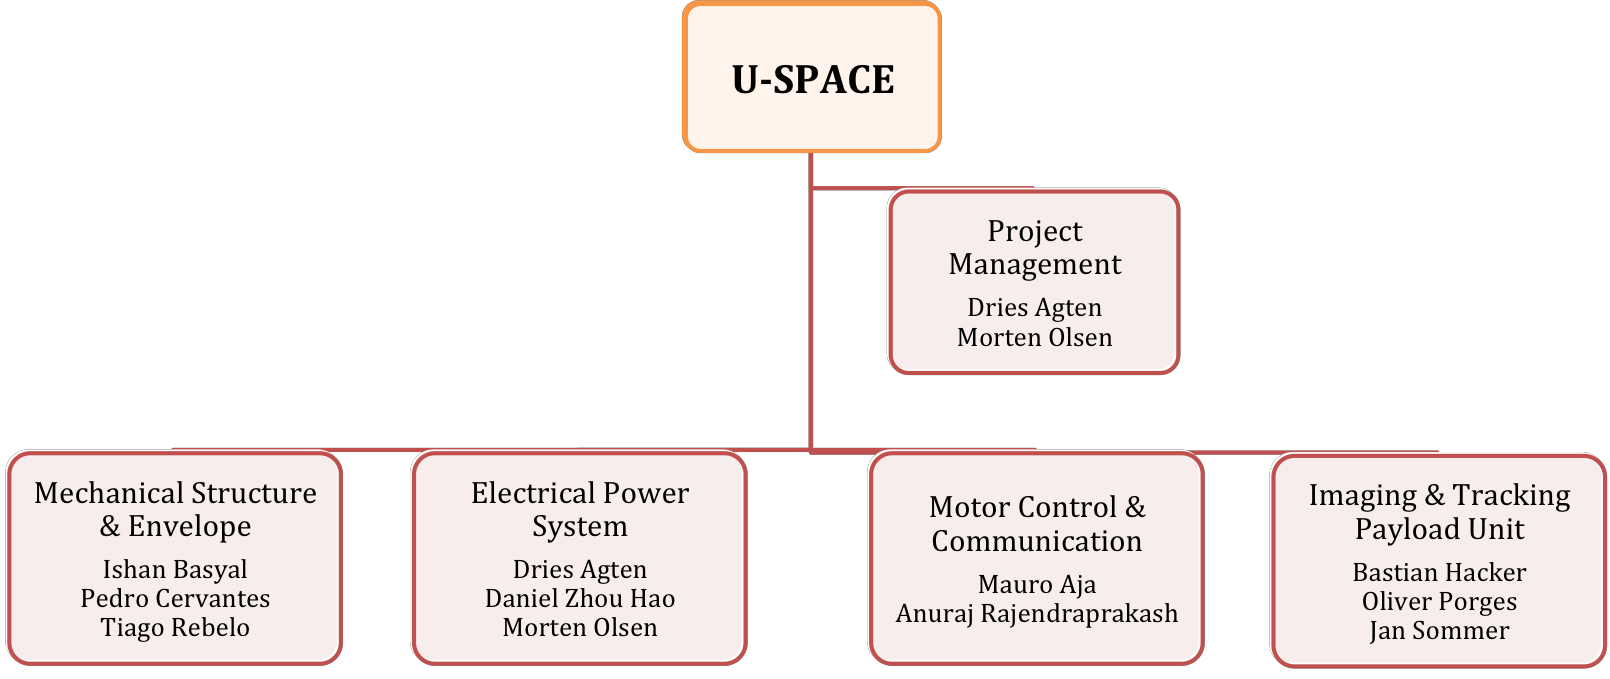
\includegraphics[width = \textwidth]{figures/obs.png} %scale=0.5
\caption{Functional organigram}
\label{fig:obs}
\end{figure}

\noindent
The background of each team member can be found in table \ref{tab:backgrounds} below.

\begin{table}[h]
\centering
\caption{Background of team members}
\begin{tabular}{l l}
\hline
\textbf{Name} & \textbf{Background} \\
\hline
Dries Agten & M.Sc. Eng. - Nanoscience \& Nanotechnology \\
Mauro Aja & B.Sc. Eng. - Electronic and Computer Engineering \\
Ishan Basyal & B.Sc. Earth and Space Sciences  \\
Pedro Cervantes & B.Sc. Eng. - Aeronautical Engineering \\
Bastian Hacker & B.Sc. Physics\\
Daniel Zhou Hao & B.Sc. Eng. - Aerospace Engineering\\
Morten Olsen & B.Sc. Eng. - Electrical Engineering \\
Oliver Porges & B.Sc. Cybernetics and Measurement  \\
Anuraj Rajendraprakash & B.Tech. Electronics Engineering \\
Tiago Rebelo & B.Sc. Eng. - Aeronautical Engineering \\
%Ivan Sinkarenko & B.Sc. Computer Science \\
Jan Sommer & B.Sc. Computational Science \\
\hline
\end{tabular}
\label{tab:backgrounds}
\end{table}

\subsection{Support Facilities}

The \ac{U-SPACE} project is supported practically, financially and technically by \ac{LTU}. \ac{IRF} and Esrange both provide technical assistance. The practical support from \ac{LTU} consists of the availability of tools and specific rooms (e.g. mechanical workshop or electronics laboratory). Also component orderning (see section \ref{subsec:ordering}) is the responsability of \ac{LTU}. The financial support is discussed in section \ref{sec:financing}.
\\
\\
The technical help of all three support entities consists of guidance regarding the components, support during the fabrication and assistance with the future testing procedures.

%\subsection{Shipment}

%Might be useful to already give it some thought...

\section{Relation With Support Facilities}

\subsection{Reporting and Monitoring}

During the entire project, the team is monitored by Kjell Lundin (\ac{IRF}) and Alf Wikström (Esrange). The team and the supervisors have weekly status meetings, in which all current issues are identified, discussed and solved. Reports to the supervisors are discussed in the next subsection.

\subsection{Reviews}

\textit{Will be included in the final version...}

\subsection{Component Ordering}
\label{subsec:ordering}

\ac{LTU} helps the team with the ordering of all components, both national and international. The procedure include component selection by the team, followed by approval of the supervisors and then the final ordering of the components by \ac{LTU}.

\section{Financing}
\label{sec:financing}

\textit{Will be included in the final version...}

\section{Schedule and Milestones}

\textit{Will be included in the final version...}

\section{Configuration Control}

%How are design changes tracked and discussed?
\textit{Will be included in the final version...}

\section{Deliverables}

\textit{Will be included in the final version...}

\subsection{Hardware and Software}

\subsection{Documentation}

\subsection{Deliverable Items and Build Standard}

%Not absolutely clear what this means... Morten?